%----------------------------------------------------------------------------------------
%	PACKAGES AND OTHER DOCUMENT CONFIGURATIONS
%----------------------------------------------------------------------------------------

\documentclass[a0,portrait]{a0poster}

\usepackage{multicol} % This is so we can have multiple columns of text side-by-side
\columnsep=100pt % This is the amount of white space between the columns in the poster
\columnseprule=3pt % This is the thickness of the black line between the columns in the poster

\usepackage[svgnames]{xcolor} % Specify colors by their 'svgnames', for a full list of all colors available see here: http://www.latextemplates.com/svgnames-colors

\usepackage{times} % Use the times font
%\usepackage{palatino} % Uncomment to use the Palatino font

\usepackage{graphicx} % Required for including images
\graphicspath{{figures/}} % Location of the graphics files
\usepackage{booktabs} % Top and bottom rules for table
\usepackage[font=small,labelfont=bf]{caption} % Required for specifying captions to tables and figures
\usepackage{amsfonts, amsmath, amsthm, amssymb} % For math fonts, symbols and environments
\usepackage{wrapfig} % Allows wrapping text around tables and figures
\usepackage[export]{adjustbox}

\begin{document}

%----------------------------------------------------------------------------------------
%	POSTER HEADER 
%----------------------------------------------------------------------------------------

% The header is divided into two boxes:
% The first is 75% wide and houses the title, subtitle, names, university/organization and contact information
% The second is 25% wide and houses a logo for your university/organization or a photo of you
% The widths of these boxes can be easily edited to accommodate your content as you see fit

\begin{minipage}[t]{0.75\linewidth}
\VeryHuge \color{HoGentAccent1} \textbf{Front end performantie in React gebaseerde applicaties} \color{Black}\\ % Title
%\Huge\textit{Ondertitel (eventueel)}\\[2.4cm] % Subtitle
\huge \textbf{Tison Matthias, Arvid De Meyer, Veerle Vuyge}\\[0.5cm] % Author(s)
\huge Hogeschool Gent, Valentin Vaerwyckweg 1, 9000 Gent\\[0.4cm] % University/organization
\Large \texttt{matthias.tison.w0715@student.hogent.be} \\
\end{minipage}
%
\begin{minipage}[t]{0.25\linewidth}

\includegraphics[width=13cm,right]{figures/HOGENT_Logo_Pos_rgb.png} 

\end{minipage}

\vspace{1cm} % A bit of extra whitespace between the header and poster content

%----------------------------------------------------------------------------------------

\begin{multicols}{2} % This is how many columns your poster will be broken into, a portrait poster is generally split into 2 columns

%----------------------------------------------------------------------------------------
%	ABSTRACT
%----------------------------------------------------------------------------------------

\color{HoGentAccent1} % Navy color for the abstract

\begin{abstract}
Performantie is een echte meeteenheid geworden door de grote opkomst van het web doorheen de jaren. Elk bedrijf heeft tegenwoordig een website en zien het als een uitlaat naar de klant. Dit zorgt ervoor dat deze betreffende websites de klanten moeten bekoren en voldoen aan hun noden. De performantie speelt hierbij een cruciale rol om als bedrijf een goede indruk na te laten bij potentiële en reeds klanten. \\
Het is voor een bedrijf dat zich specialiseert in web- en native applicaties een absoluut werkpunt bij elk project dat ze aangaan. Dit wordt nog groter wanneer het gaat over complexe applicaties. \\
React heeft zich mee ontbolsterd tijdens de modernisering van het web. Er was een eerste teken van React in begin 2010 en tot nu toe heeft het enkel meer zijn voetafdruk gezet op vlak van front end applicaties. Daaropvolgend betekend het ook dat het de meeste performantie struikelblokken weet aan te pakken op een efficiënte manier.
\end{abstract}
%----------------------------------------------------------------------------------------
%	INTRODUCTION
%----------------------------------------------------------------------------------------

\color{HoGentAccent1} 
\section*{Introductie}
\color{black}
\color{black}
Het onderzoek in deze scriptie verdiept zich in de impact van performantie en hoe deze te optimaliseren, binnen het React framework. De meest prominente methoden worden aangehaald en uitgewerkt. Uiteraard zijn mogelijkheden voor optimalisatie niet gelimiteerd tot het framework zelf en wordt er onderzocht welke mogelijkheden zich aanbieden buiten React. \\
Dat terzijde moet er voor optimalisatie eerst kennis vergaard worden over wat performantie daadwerkelijk inhoud en hoe we het meten. Cruciaal voor optimalisatie is het onderzoeken van knelpunten binnen de applicatie door metingen te verrichten en op basis daarvan te handelen. \\
Het doel van dit onderzoek is om juiste optimalisatie methoden toe te kunnen passen waar nodig, zowel binnen als buiten de React codebase.

%----------------------------------------------------------------------------------------
%	EXPERIMENTEN
%----------------------------------------------------------------------------------------

\color{Black} % DarkSlateGray color for the rest of the content
\color{HoGentAccent1} 
\section*{Uitwerkingen}
\color{black}

De uitwerkingen zijn onderverdeeld in 2 blokken. Er wordt een onderscheid gemaakt tussen het theoretische en praktische. In de theorie komt de impact en metrieken van performantie aan bod. Daarna is het praktische onderverdeeld in 3 onderdelen. \\
Het eerste deel onderzoekt methoden van React zelf en gebruikt kunnen worden door middel van de React API. Tweede deel haalt methoden aan die door gebruik van het framework mogelijk zijn. Tenslotte zijn er de methoden die aangeboden worden los van het framework en de React API.

\color{HoGentAccent1} 
\section*{Sectie met figuren}
\color{black}

\begin{center}\vspace{1cm}
    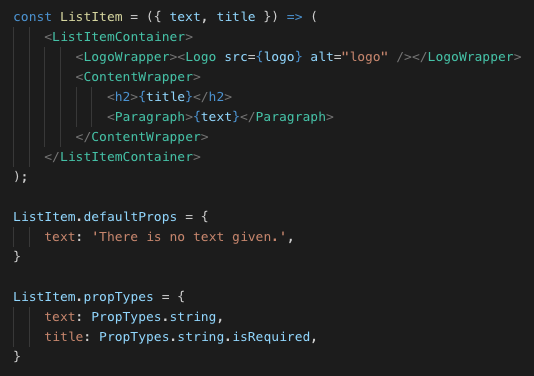
\includegraphics[width=1.0\linewidth]{ComponentWithProps}
    \captionof{figure}{\color{HoGentAccent5} Functioneel component binnen React}
\end{center}\vspace{1cm}

\begin{center}\vspace{1cm}
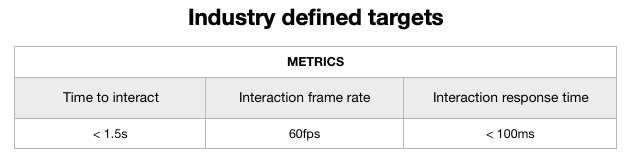
\includegraphics[width=1.0\linewidth]{InteractionSpeedTarget}
\captionof{figure}{\color{HoGentAccent5} Industrie snelheid standaarden}
\end{center}\vspace{1cm}

\begin{center}\vspace{1cm}
    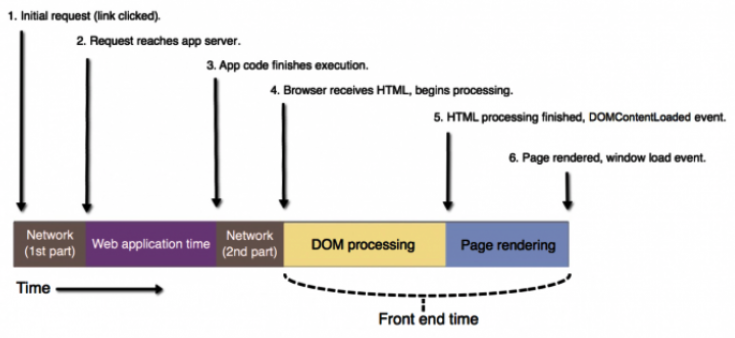
\includegraphics[width=1.0\linewidth]{BrowserPageLoadTimeline}
    \captionof{figure}{\color{HoGentAccent5} Laad proces van een pagina}
\end{center}\vspace{1cm}

%------------------------------------------------

\color{HoGentAccent1} 
\section*{Conclusies}
\color{black}

De conclusies uit het onderzoek geven aan dat er voor optimalisatie een significante analyse moet gedaan worden van de knelpunten in verband met performantie. Verder kan uit het onderzoek geconcludeerd worden dat React een beduidend aantal mogelijkheden biedt voor performantie optimalisatie. Ook buiten React zijn er vele methoden om tot merkbare optimalisatie te komen. \\
Er valt ook te concluderen dat het niet eenvoudig is om zelf een significante belasting te leggen op een website voor het testen van performantie methoden.

%----------------------------------------------------------------------------------------
%	FORTHCOMING RESEARCH
%----------------------------------------------------------------------------------------
\color{HoGentAccent1} 
\section*{Toekomstig onderzoek}
\color{black}

Technologie en programmeren in het algemeen zal in de toekomst nog meer wendingen nemen. Die wendingen zullen ook telkens weer mogelijkheden bieden voor nieuw onderzoek in zaken performantie. Standaarden zullen hoger komen te liggen en nieuwe innovatieve manieren komen ter sprake. Ook dan is het noodzakelijk om deze methoden te onderzoeken en hun voordelen en de toepassing ervan aan te halen. \\
React maakte onlangs nog een wending door de introductie van React Hooks en zo zullen er nog volgen.

%----------------------------------------------------------------------------------------

\end{multicols}
\end{document}